\subsection{Opis implementacji}
Dokonano implementacji trzech funkcjonalności odpowiadających kolejnym krokom przeprowadzonym w tej pracy. Pierwszym z nich jest pobranie danych, następnie ich analiza a na koniec przeprowadzenie klasyfikacji danych. Poniżej przedstawiono opis przygotowania projektu oraz implementacji stworzonych rozwiązań. 
\subsubsection{Pobieranie danych}
Aby dokonać pobrania danych stworzono system informatyczny dedykowany do tego zadania. Użyto w tym celu języka Java z zastosowaniem framework Spring Boot. Podjęto taką decyzje ponieważ jest to język dostosowany do zadania jakim jest wysyłanie zapytań do zewnętrznego api oraz zapisywanie danych do baz danych oraz jest dobrze znany autorowi.

Dla ułatwienia pracy przy korzystaniu z\,Twitter API\footnote{\url{http://twitter4j.org}} użyto ogólnodostępną bibliotekę Twitter4J stworzoną dla języka Java i\,objętą licencją Apache Licence 2.0. Biblioteka ta udostępnia klasy oraz metody wspomagające integrację nowej aplikacji z\,serwisem Twitter. Dzięki jej zaadoptowaniu w\,nowej aplikacji nie musiały znaleźć się bezpośrednie zapytania http co zwiększyło czytelność kodu. Twitter API spełnia zasady stylu architektonicznego REST. Dzięki użyciu odpowiednich metod pochodzących z biblioteki wystarczy podać odpowiednie parametry do metody, aby wykonać zapytanie do zewnętrznego serwera.
\par
Zebrane dane zapisywano do lokalnej bazy danych PostgreSQL. Jest to jedna z najpopularniejszych darmowych relacyjnych baz danych. W celu zapisania informacji do bazy danych stworzono odpowiednie encje. Biblioteka Twitter4J posiada swoje obiekty odpowiadające strukturom odpowiedzi z Twitter API, jednak w systemie należało stworzyć własne. Jest tak z dwóch powodów. Pierwszym z nich jest fakt, że klasy biblioteki Twitter4J posiadały dużo atrybutów, które wiadomo było, że są nieznaczące dla dalszej analizy. Drugim powodem był fakt, że należało dodać kilka dodatkowych atrybutów, aby ułatwić dalszą analizę. Takimi atrybutami były na przykład liczniki zebranych obiektów. Warto wspomnieć, że wybierając atrybuty dla encji starano się wybrać wszystkie, które mogą być przydatne w przyszłej analizie. Diagram relacji  wraz z atrybutami encji został przedstawiony na rysunku \ref{fig:diagram-db}
\begin{figure}[!h]
	\centering 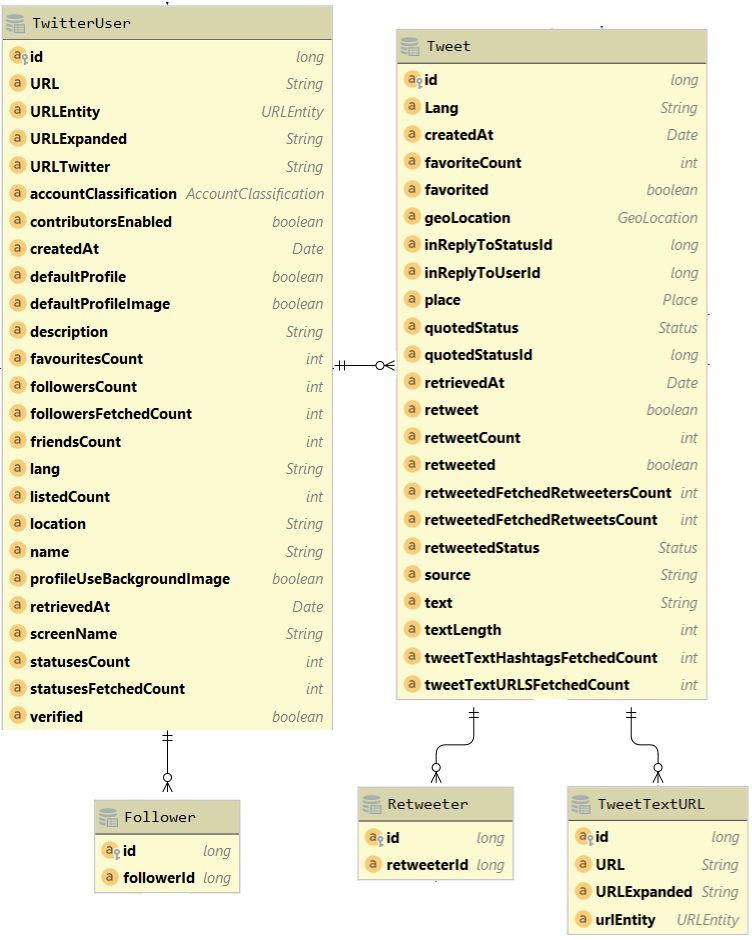
\includegraphics[width=0.9\linewidth]{img/diagramERD.png}
	\caption{Diagram ERD bazy danych. } \label{fig:diagram-db}
\end{figure}
\par
\par
Implementując rozwiązanie pobierania danych rozpisano je na odpowiednie kroki. Składają się one z trzech głównych faz: wykonanie zapytania do Twitter API korzystając z metod biblioteki Twitter4J, utworzenie odpowiednich obiektów i ich relacji, zapisanie danych w badzie danych. Aby tego dokonać użyto wzorca wykorzystującego ideę warstw serwisu oraz repozytorium. Serwisy obsługują logikę potrzebną do odpowiedniego przetwarzania danych. 

\par
Należało również pamiętać o ograniczeniach wiążących się z liczbą wysyłanych zapytań. W tym celu musiano usypiać wątek po każdym wykonanym zapytaniu na określony czas aby łącznie nie przekroczyć maksymalnej liczby wywołań w określonej jednostce czasu. 

\par
Dodatkowo wykorzystano ten samą aplikację w celu przygotowania danych do analizy. Posiadając odpowiednie struktury encji, dodano kolejne klasy odpowiadające typom danych jakie będą użyteczne w trakcie analizy. Stworzono w tym celu również pakiet nowych serwisów których celem było przetwarzanie zgromadzonych w bazie danych informacji w formę odpowiednią do analizy. Wykorzystano w tym celu głównie zapytania SQL używając framework Spring Data JPA. Działano w ten sposób ze względu na szybkość selekcji oraz agregacji danych które były kluczowe przy pracy z dużą liczbą danych. 

\par
% poprawic diagrm

% opisac jakie typy danych
% opisac entity repository service

% opisac odpowiednie zabezpieczenia (sleep) aby dotrzymac ograniczeniom